\documentclass[border=5mm]{standalone}
\usepackage{xcolor}
\usepackage{tikz}
\usetikzlibrary{positioning}
\usetikzlibrary{calc}
\begin{document}

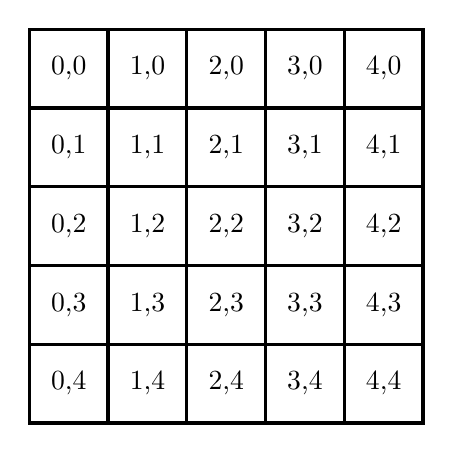
\begin{tikzpicture}
    [%%%%%%%%%%%%%%%%%%%%%%%%%%%%%%
        box/.style={rectangle,draw=black,very thick, minimum size=1cm}
    ]%%%%%%%%%%%%%%%%%%%%%%%%%%%%%%

\foreach \x in {0,1,...,4}{
    \foreach \y in {0,1,...,4}
    {
        \pgfmathsetmacro{\r}{int(4-\y)}
        \node[box] at (\x,\y){ \x,\r};
    }
}

\end{tikzpicture}
\end{document}